%%%%%%%%%%%%%%%%%%%%%%%%%%%%%%%%%%%%%%%%%
% Beamer Presentation
% LaTeX Template
% Version 1.0 (10/11/12)
%
% This template has been downloaded from:
% http://www.LaTeXTemplates.com
%
% License:
% CC BY-NC-SA 3.0 (http://creativecommons.org/licenses/by-nc-sa/3.0/)
%
%%%%%%%%%%%%%%%%%%%%%%%%%%%%%%%%%%%%%%%%%

%----------------------------------------------------------------------------------------
%	PACKAGES AND THEMES
%----------------------------------------------------------------------------------------

\documentclass{beamer}

\mode<presentation> {

% The Beamer class comes with a number of default slide themes
% which change the colors and layouts of slides. Below this is a list
% of all the themes, uncomment each in turn to see what they look like.

%\usetheme{default}
%\usetheme{AnnArbor}
%\usetheme{Antibes}
%\usetheme{Bergen}
%\usetheme{Berkeley}
%\usetheme{Berlin}
%\usetheme{Boadilla}
\usetheme{CambridgeUS}
%\usetheme{Copenhagen}
%\usetheme{Darmstadt}
%\usetheme{Dresden}
%\usetheme{Frankfurt}
%\usetheme{Goettingen}
%\usetheme{Hannover}
%\usetheme{Ilmenau}
%\usetheme{JuanLesPins}
%\usetheme{Luebeck}
%\usetheme{Madrid}
%\usetheme{Malmoe}
%\usetheme{Marburg}
%\usetheme{Montpellier}
%\usetheme{PaloAlto}
%\usetheme{Pittsburgh}
%\usetheme{Rochester}
%\usetheme{Singapore}
%\usetheme{Szeged}
%\usetheme{Warsaw}

% As well as themes, the Beamer class has a number of color themes
% for any slide theme. Uncomment each of these in turn to see how it
% changes the colors of your current slide theme.

%\usecolortheme{albatross}
%\usecolortheme{beaver}
%\usecolortheme{beetle}
%\usecolortheme{crane}
%\usecolortheme{dove}
%\usecolortheme{fly}
%\usecolortheme{seagull}
%\usecolortheme{wolverine}
%Outer color themes
%\usecolortheme{dolphin}
%\usecolortheme{seahorse}
%\usecolortheme{whale}
%Inner color themes
%\usecolortheme{lily}
%\usecolortheme{orchid}
%\usecolortheme{rose}

%\setbeamertemplate{footline} % To remove the footer line in all slides uncomment this line
%\setbeamertemplate{footline}[page number] % To replace the footer line in all slides with a simple slide count uncomment this line

%\setbeamertemplate{navigation symbols}{} % To remove the navigation symbols from the bottom of all slides uncomment this line
}

\usepackage{gensymb}
\usepackage{graphicx} % Allows including images
\usepackage{booktabs} % Allows the use of \toprule, \midrule and \bottomrule in tables

%----------------------------------------------------------------------------------------
%	TITLE PAGE
%----------------------------------------------------------------------------------------

% The short title appears at the bottom of every slide, the full title is only on the title page
\title[Resistor Identification]{Resistor Detection and Classification Using Support Vector Machines}

\author{David McNeil} % Your name
\institute[RHIT] % Your institution as it will appear on the bottom of every slide, may be shorthand to save space
{
Rose-Hulman Institute of Technology \\ % Your institution for the title page
\medskip
\textit{mcneilde@rose-hulman.edu} % Your email address
}
%\date{\today} % Date, can be changed to a custom date
\date{}

\begin{document}

% Print the title page as the first slide
\begin{frame}
\titlepage
\end{frame}

% Table of contents slide, comment this block out to remove it
\begin{frame}
\frametitle{Overview}
\tableofcontents % Throughout your presentation, if you choose to use \section{} and \subsection{} commands, these will automatically be printed on this slide as an overview of your presentation
\end{frame}

%----------------------------------------------------------------------------------------
%	PRESENTATION SLIDES
%----------------------------------------------------------------------------------------
% slides are 3in high by 5in wide
%------------------------------------------------
\section{Introduction} 
%------------------------------------------------

\begin{frame}
\frametitle{Objective}
\begin{columns}[c]
  \column{2.5in}
	\begin{block}{Successfully be able to detect and classify resistors in an image.}
	\begin{itemize}
		\item Detection-- Determining the location of the resistors in the image
		\item Classification-- Determining the resistor value based on color codes
	\end{itemize}
	\end{block}
  \column{1.5in}
  \frame{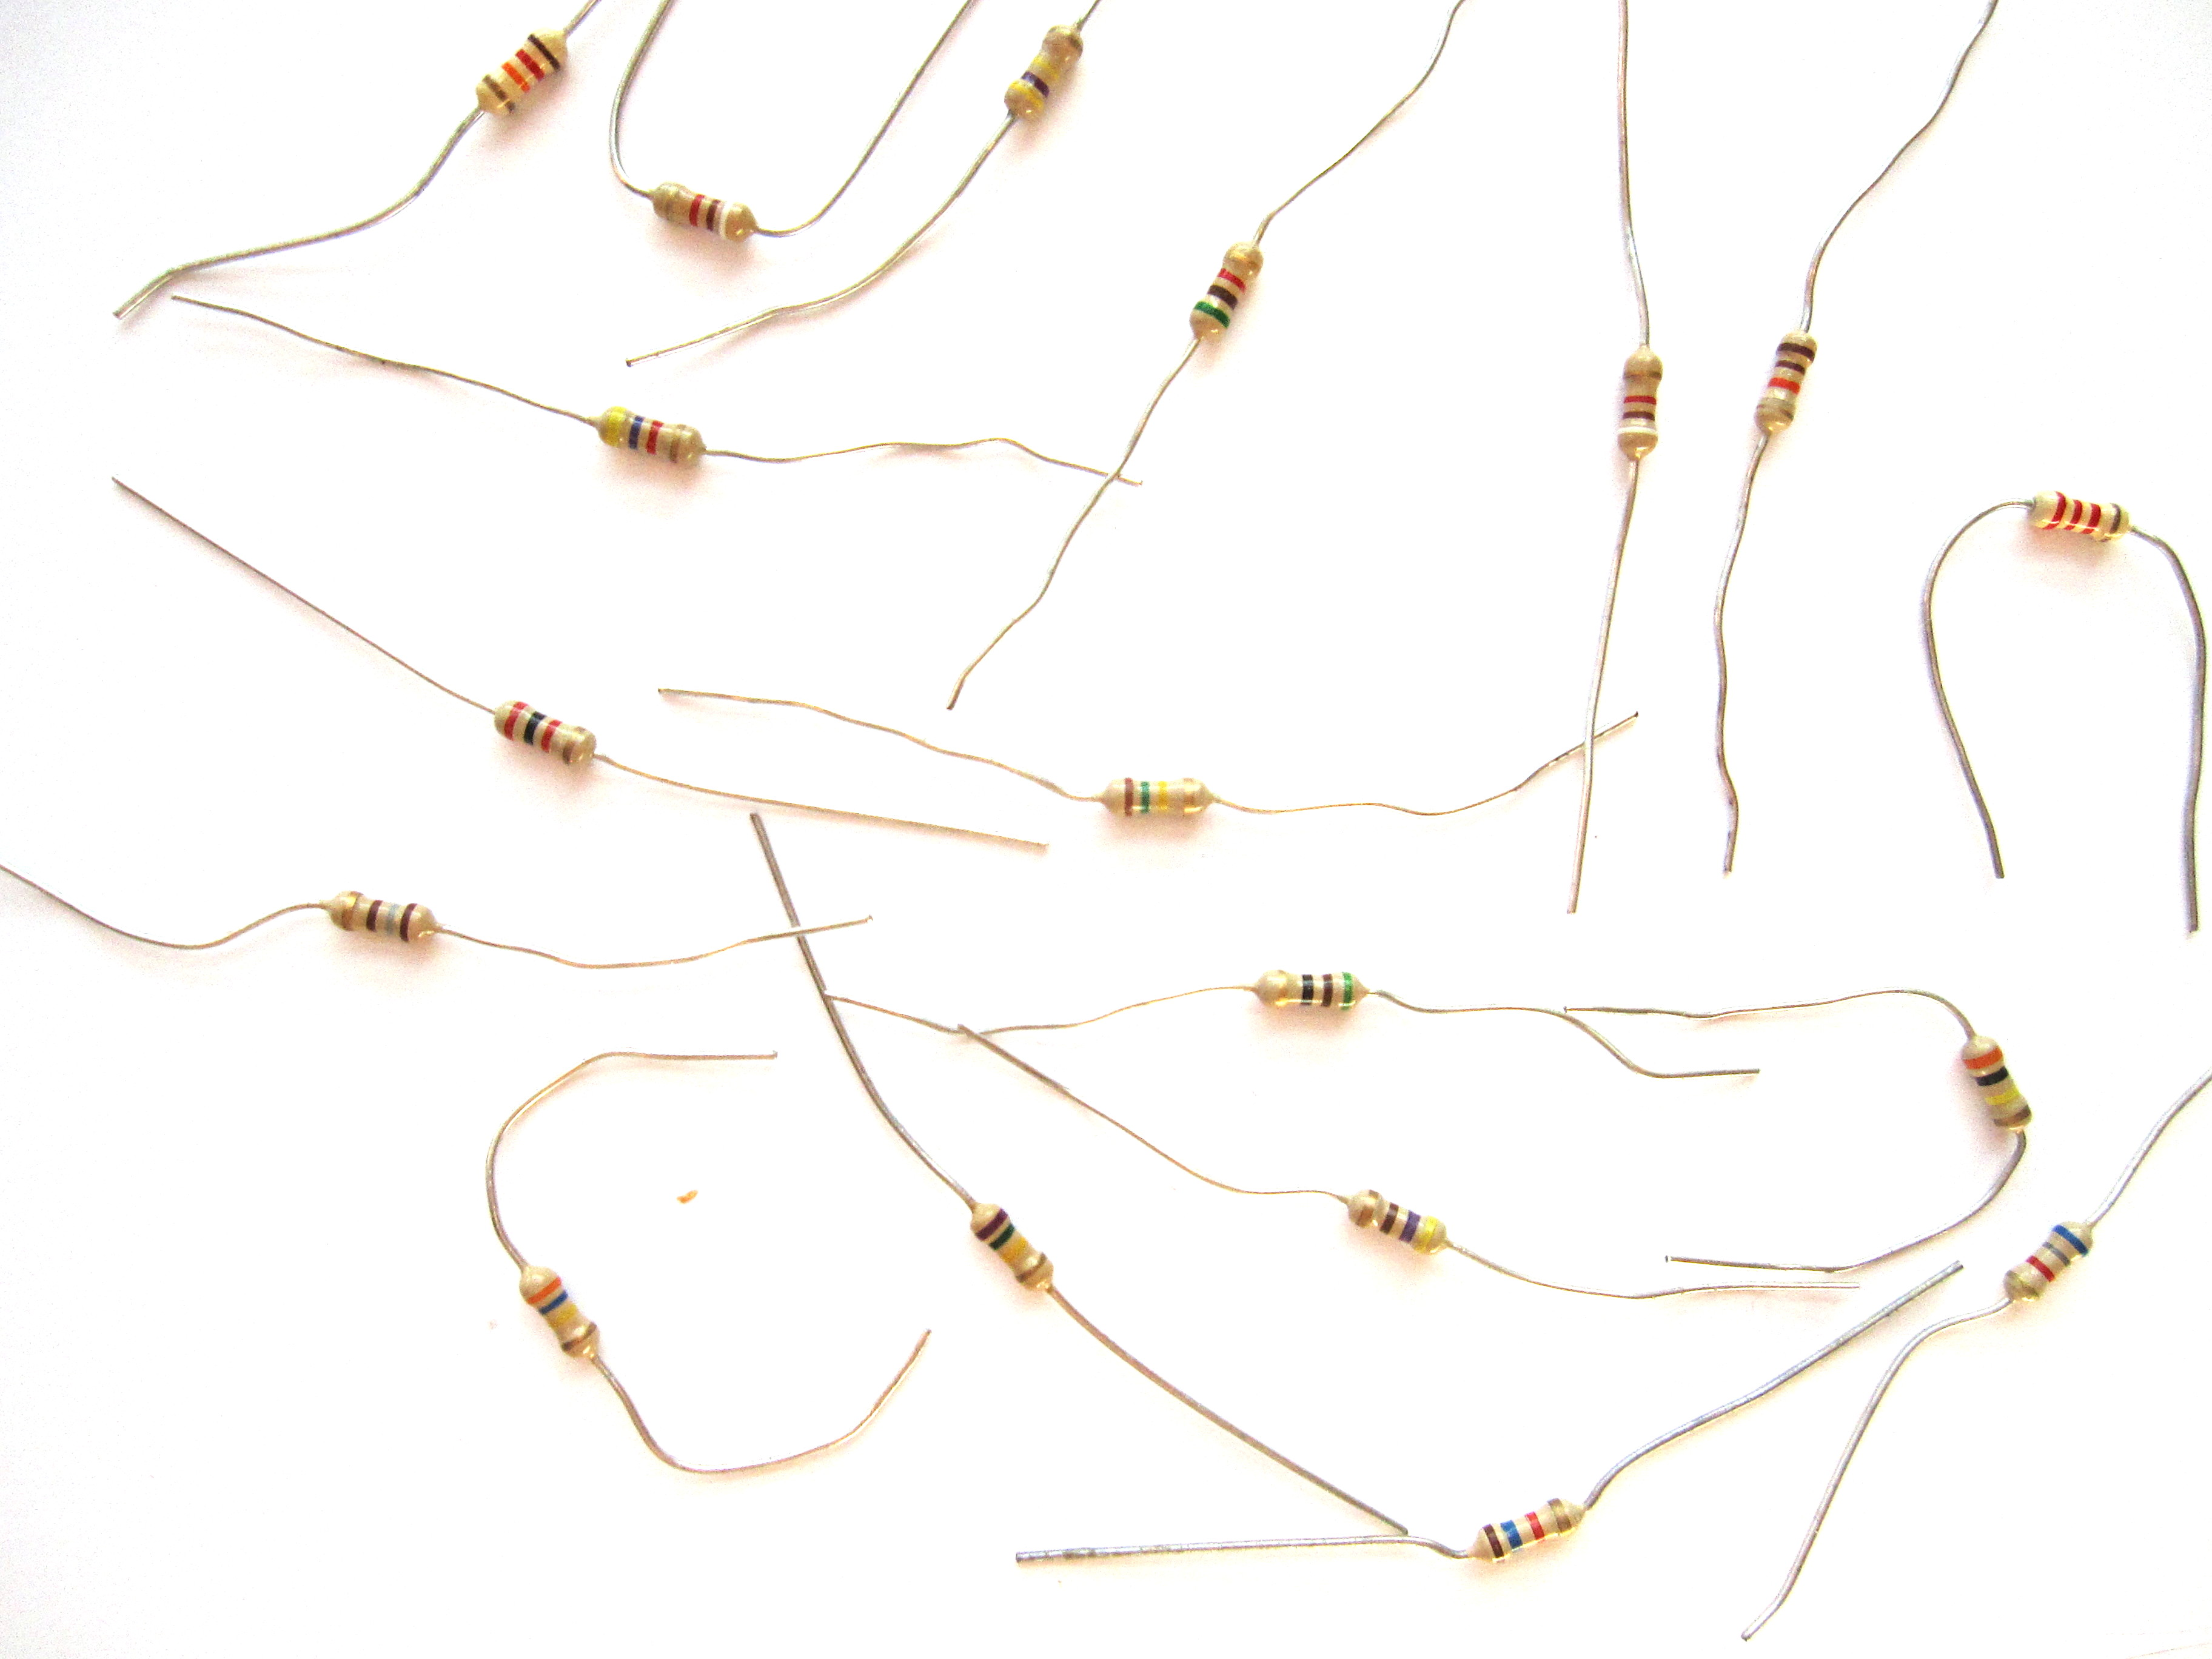
\includegraphics[width=1.5in]{images/example.jpg}}
\end{columns}
\end{frame}

%------------------------------------------------

\begin{frame}
\frametitle{Resistor Color Codes}
\begin{center}
\frame{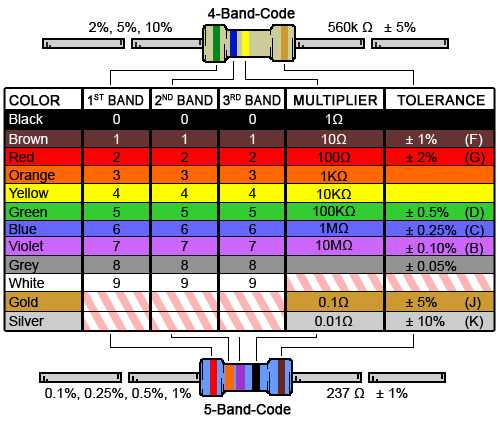
\includegraphics[width=3in]{images/resistor-color-chart.jpg}}
\end{center}
\end{frame}

%------------------------------------------------

\begin{frame}
\frametitle{Assumptions}
\begin{columns}[c]
  \column{3in}
    \begin{block}{}
	\begin{itemize}
	\item Resistors are all of a standard type
	\item Resistors are of a similar size in images
	\item Images are all of the same resolution
	\item Images have a similar white balance
	\item Images have been taken on a white background
	\item Images have been taken with a consistent camera angle
	\item Images only include resistors
	\end{itemize}
	\end{block}
  \column{1in}
  \frame{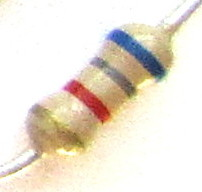
\includegraphics[width=1in]{images/resistor.jpg}}
\end{columns}
\end{frame}

%------------------------------------------------
\section{Detection} 
%------------------------------------------------

\begin{frame}
\frametitle{Detection}
\begin{block}{Basic Approach}
\begin{itemize}
\item Convert image to black and white (binary image)
\item Convolve the binary image with a binary mask of a resistor
\item Rotate the binary mask and convolve again, repeat at 10\degree intervals
\item Find local maximum in the convolved space
\end{itemize}
\end{block}
\end{frame}

%------------------------------------------------

\begin{frame}
\frametitle{Initial Image}
\begin{center}
\frame{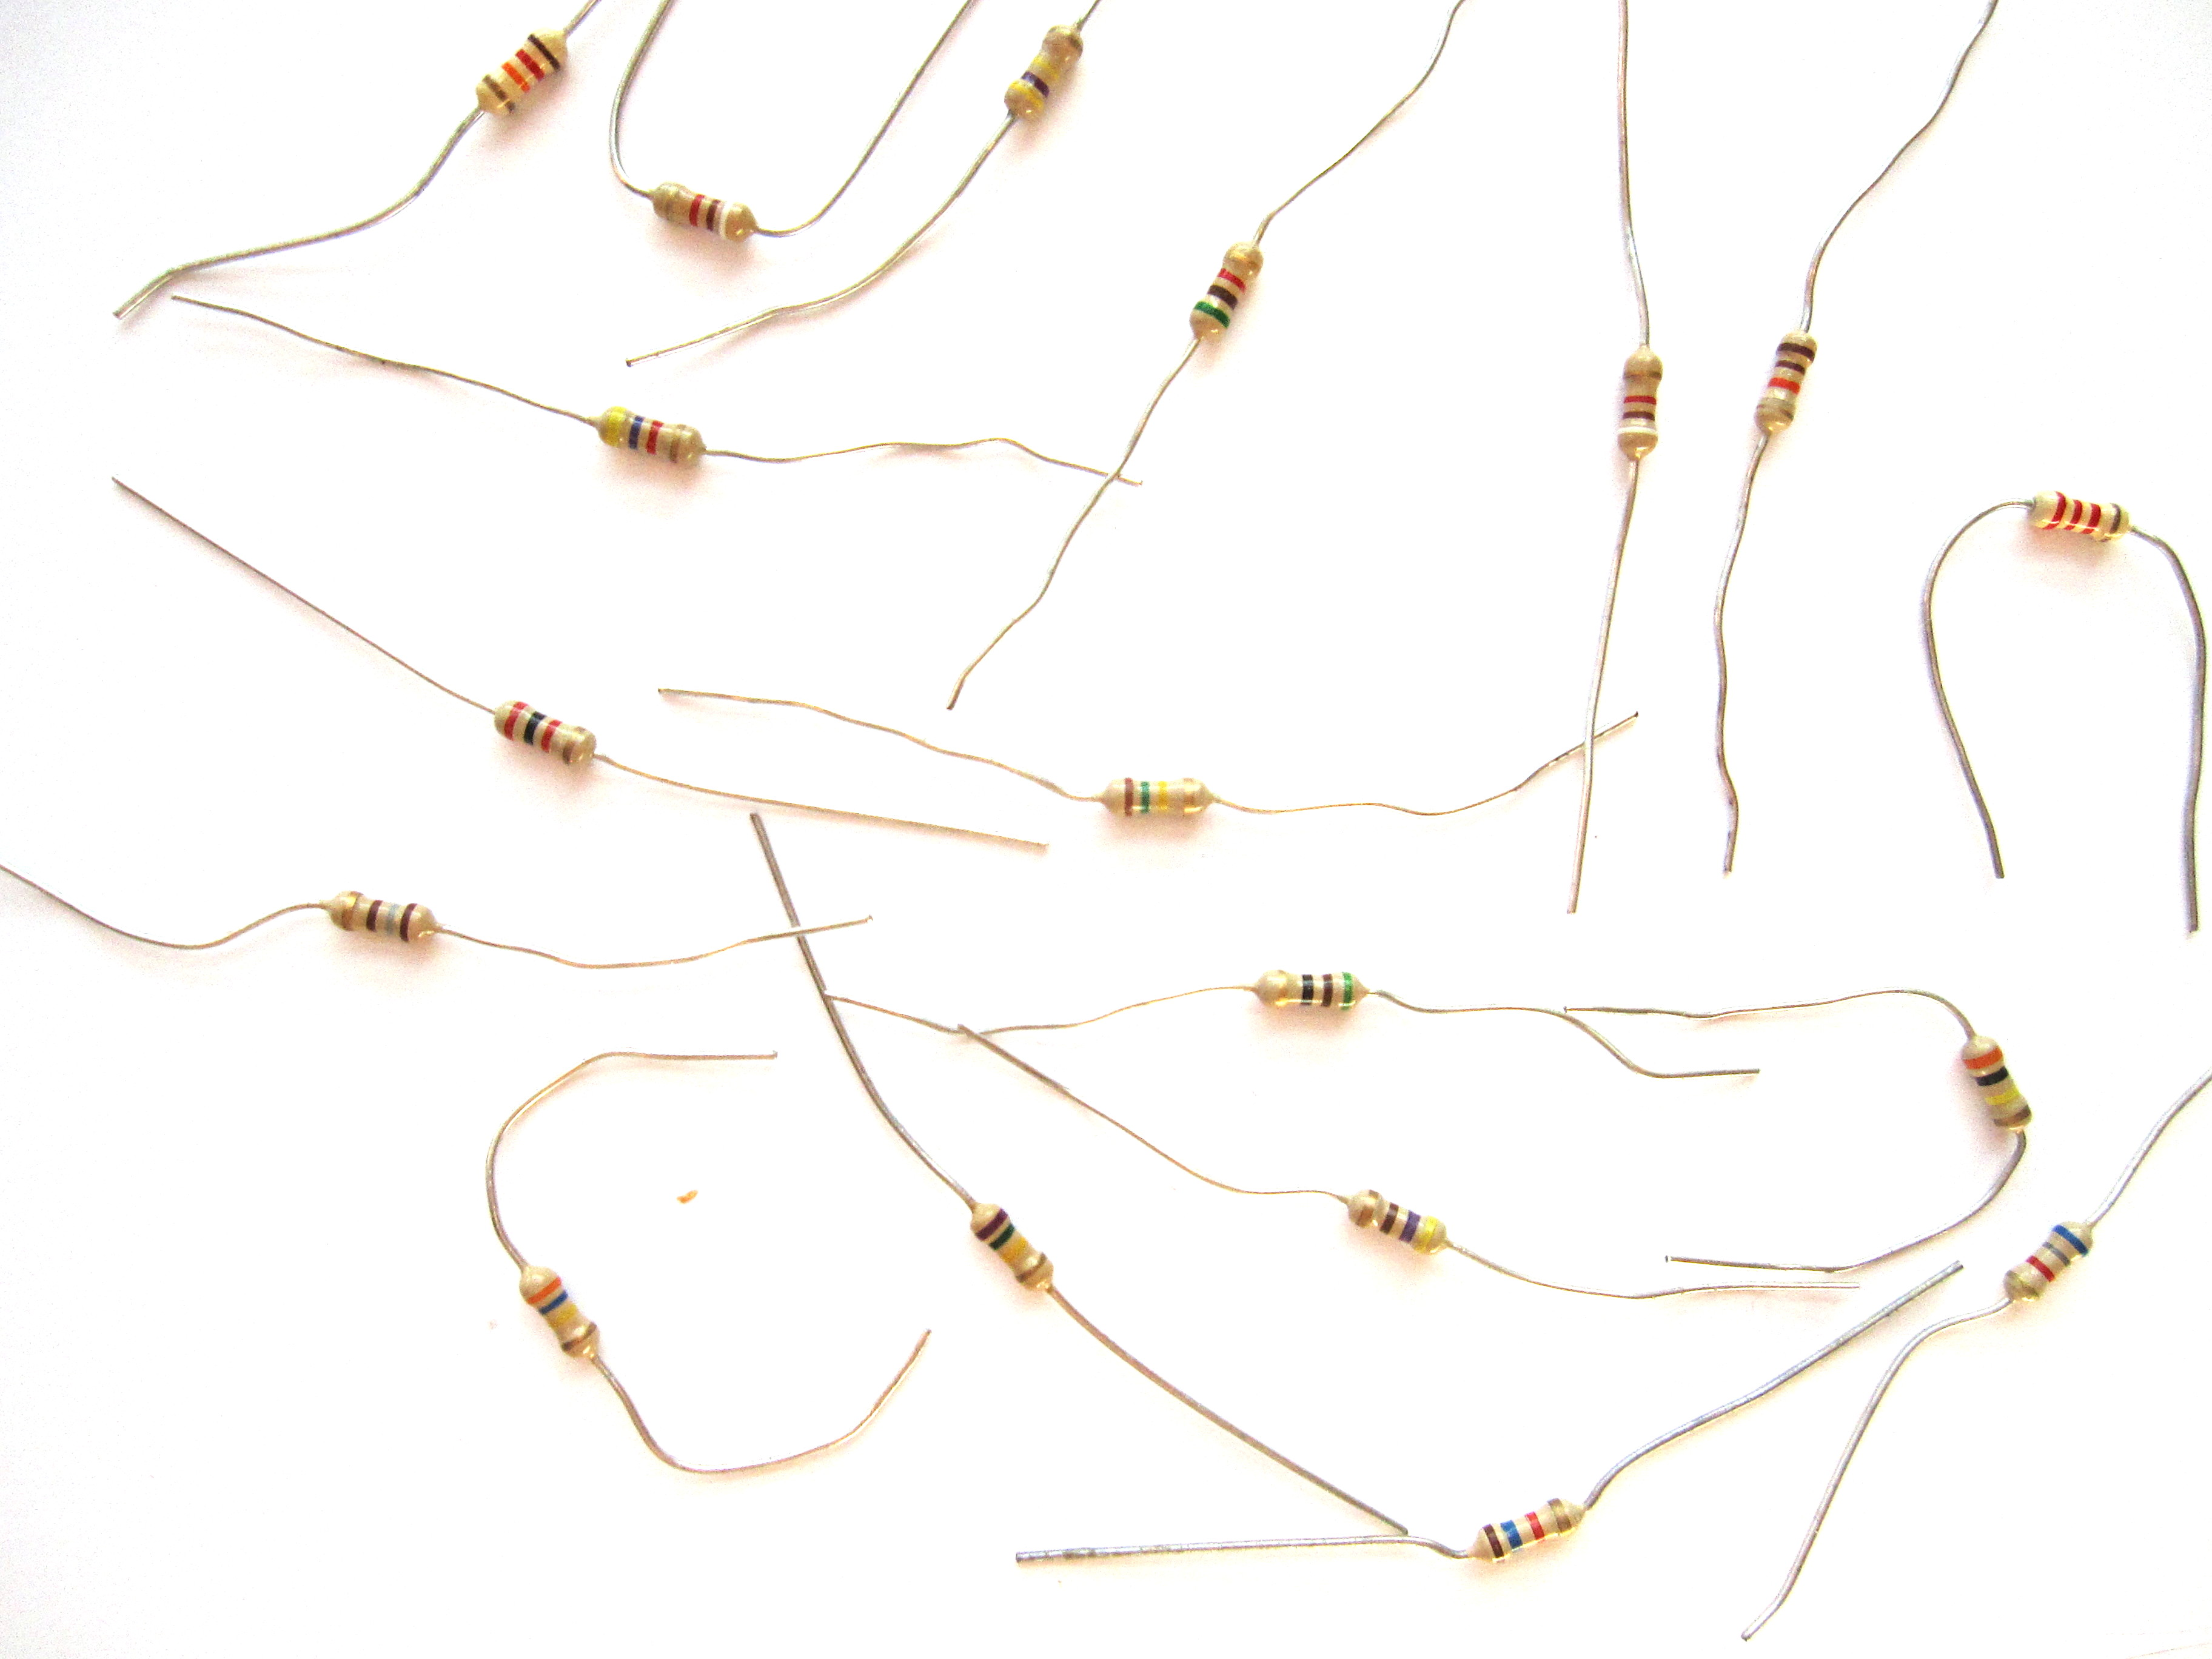
\includegraphics[width=3in]{images/example.jpg}}
\end{center}
\end{frame}

%------------------------------------------------

\begin{frame}
\frametitle{Binary Image}
\begin{center}
\frame{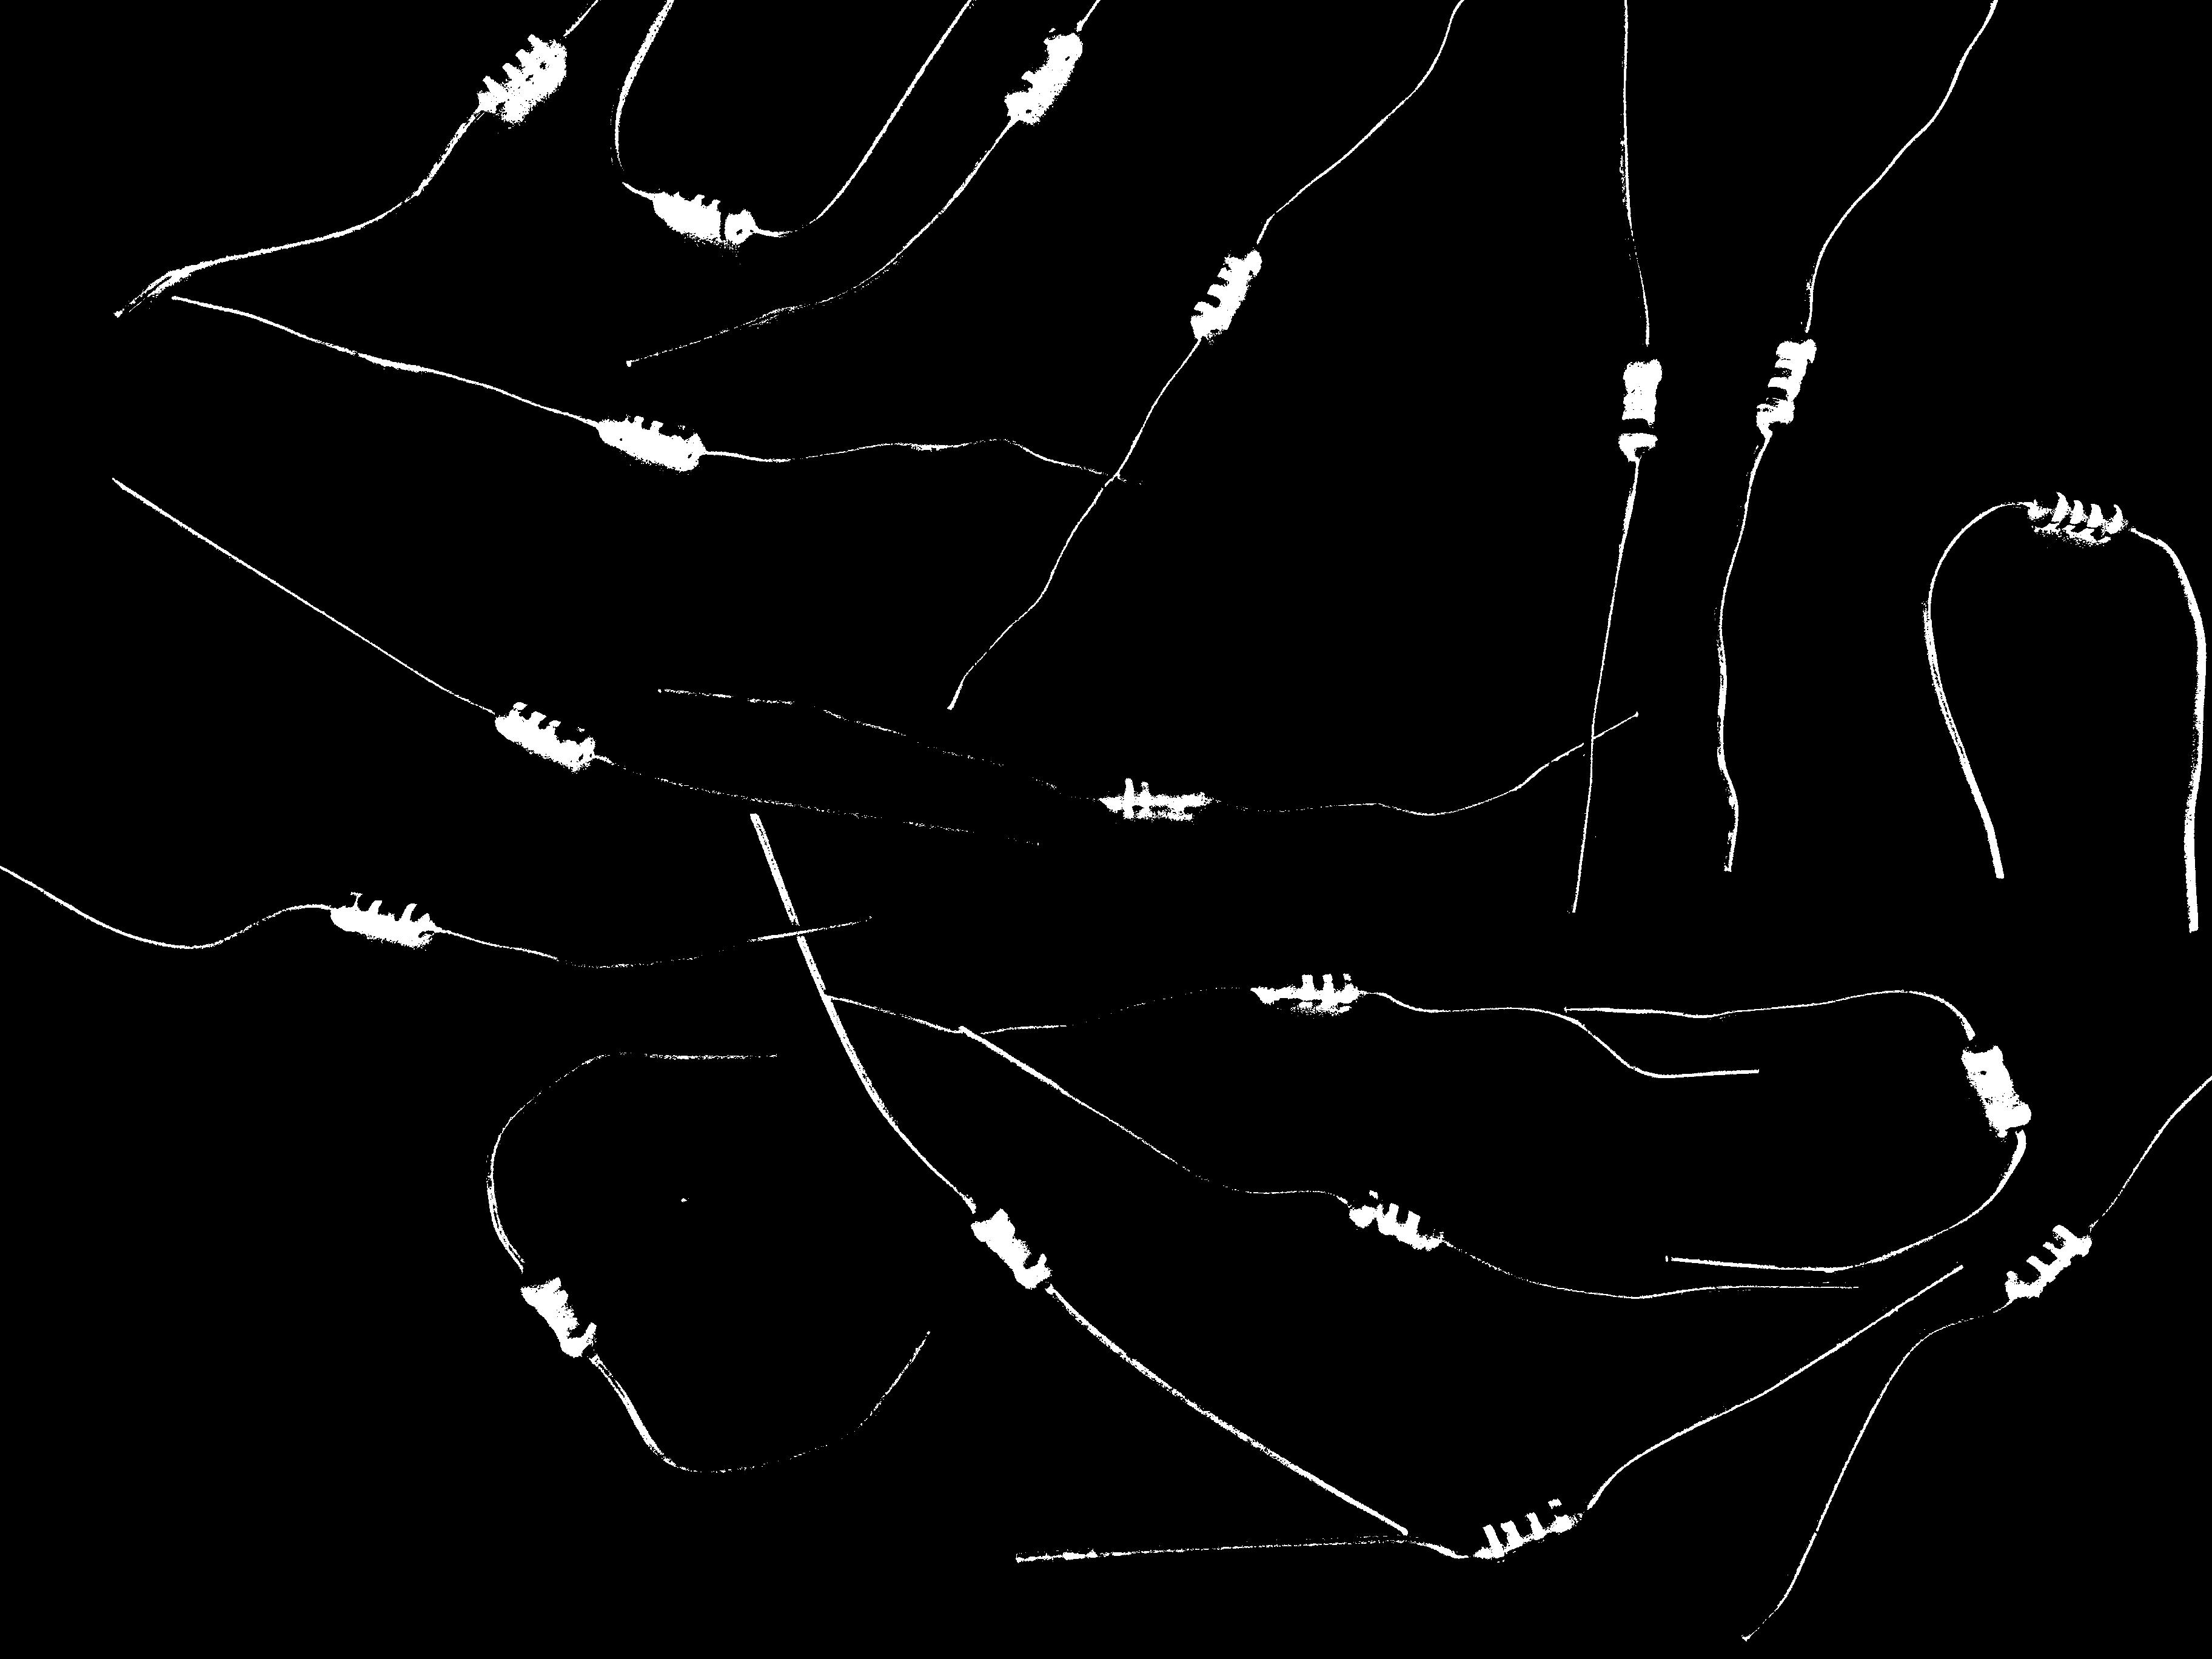
\includegraphics[width=3in]{images/Ibw.jpg}}
\end{center}
\end{frame}

%------------------------------------------------

\begin{frame}
\frametitle{Resistor Mask}
\begin{center}
\frame{
\includegraphics[width=2.25in]{images/mask.png}}
\end{center}
\end{frame}

%------------------------------------------------

\begin{frame}
\frametitle{Convolved Images}
\begin{columns}[c]
  \column{2in}
  	\begin{center}
  	Mask at 0\degree
  	\end{center}
	\frame{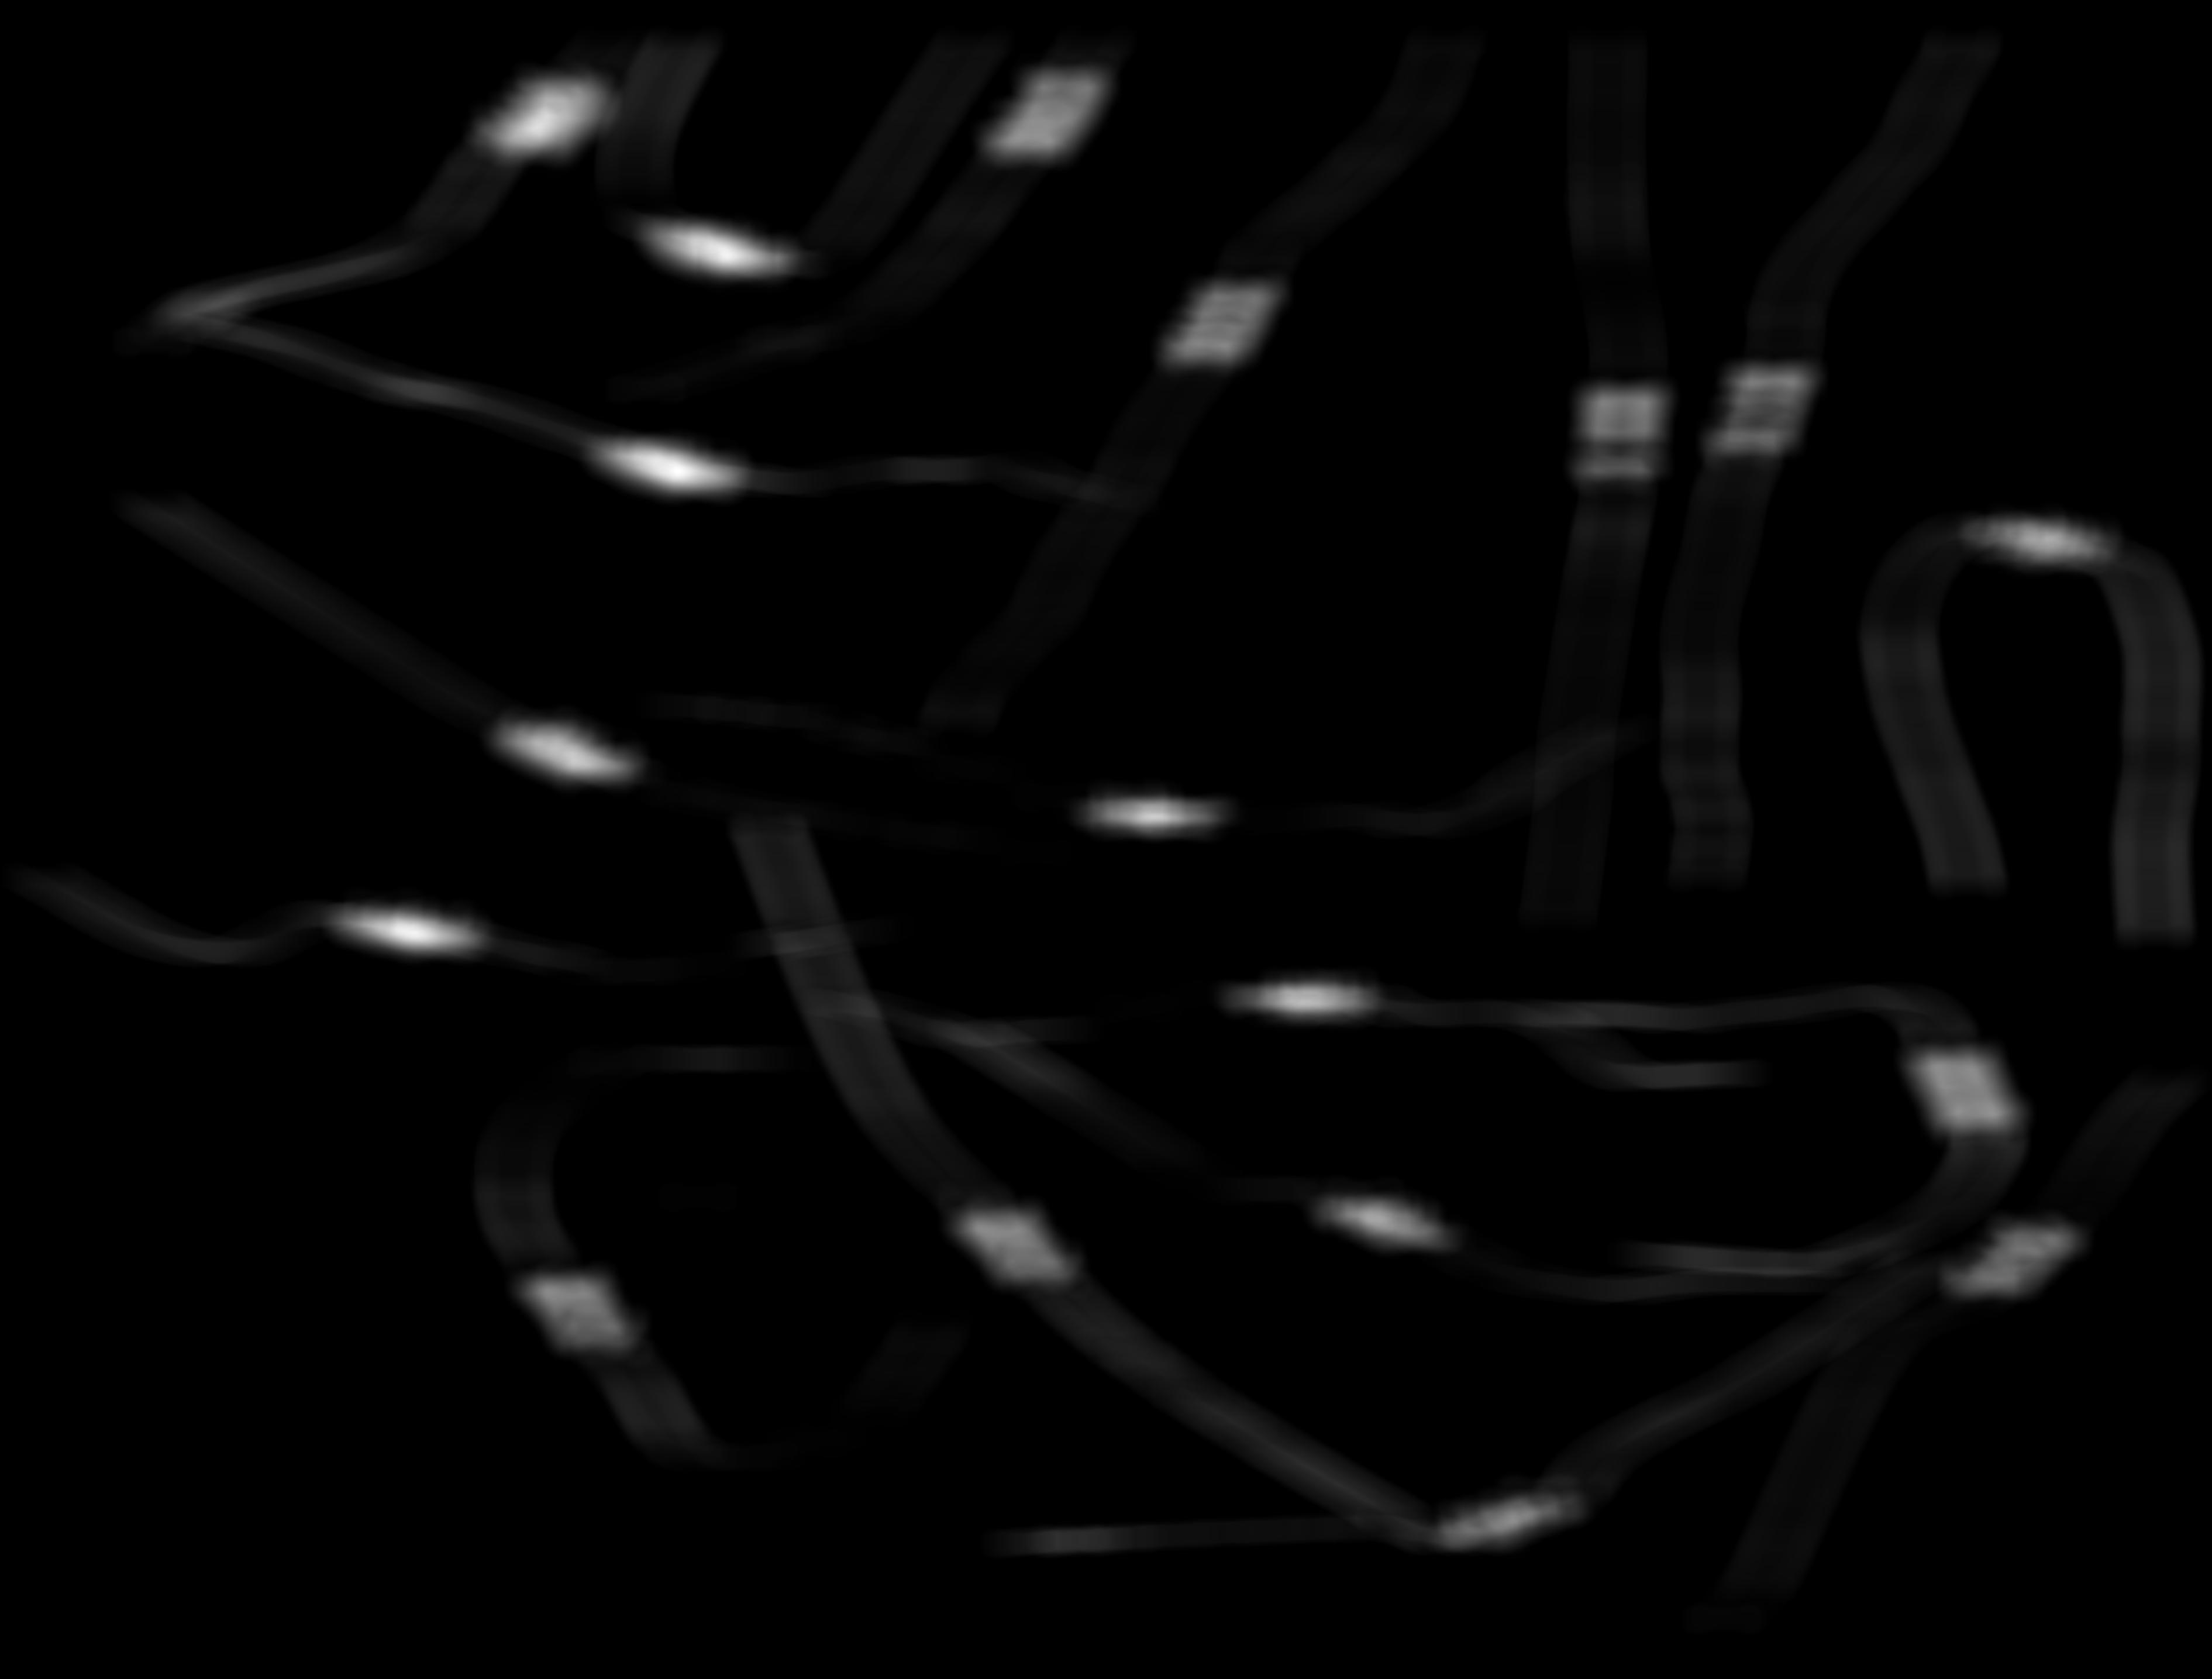
\includegraphics[width=2.2in]{images/conv0.jpg}}
  \column{2in}
    \begin{center}
  	Mask at 90\degree
  	\end{center}
  	\frame{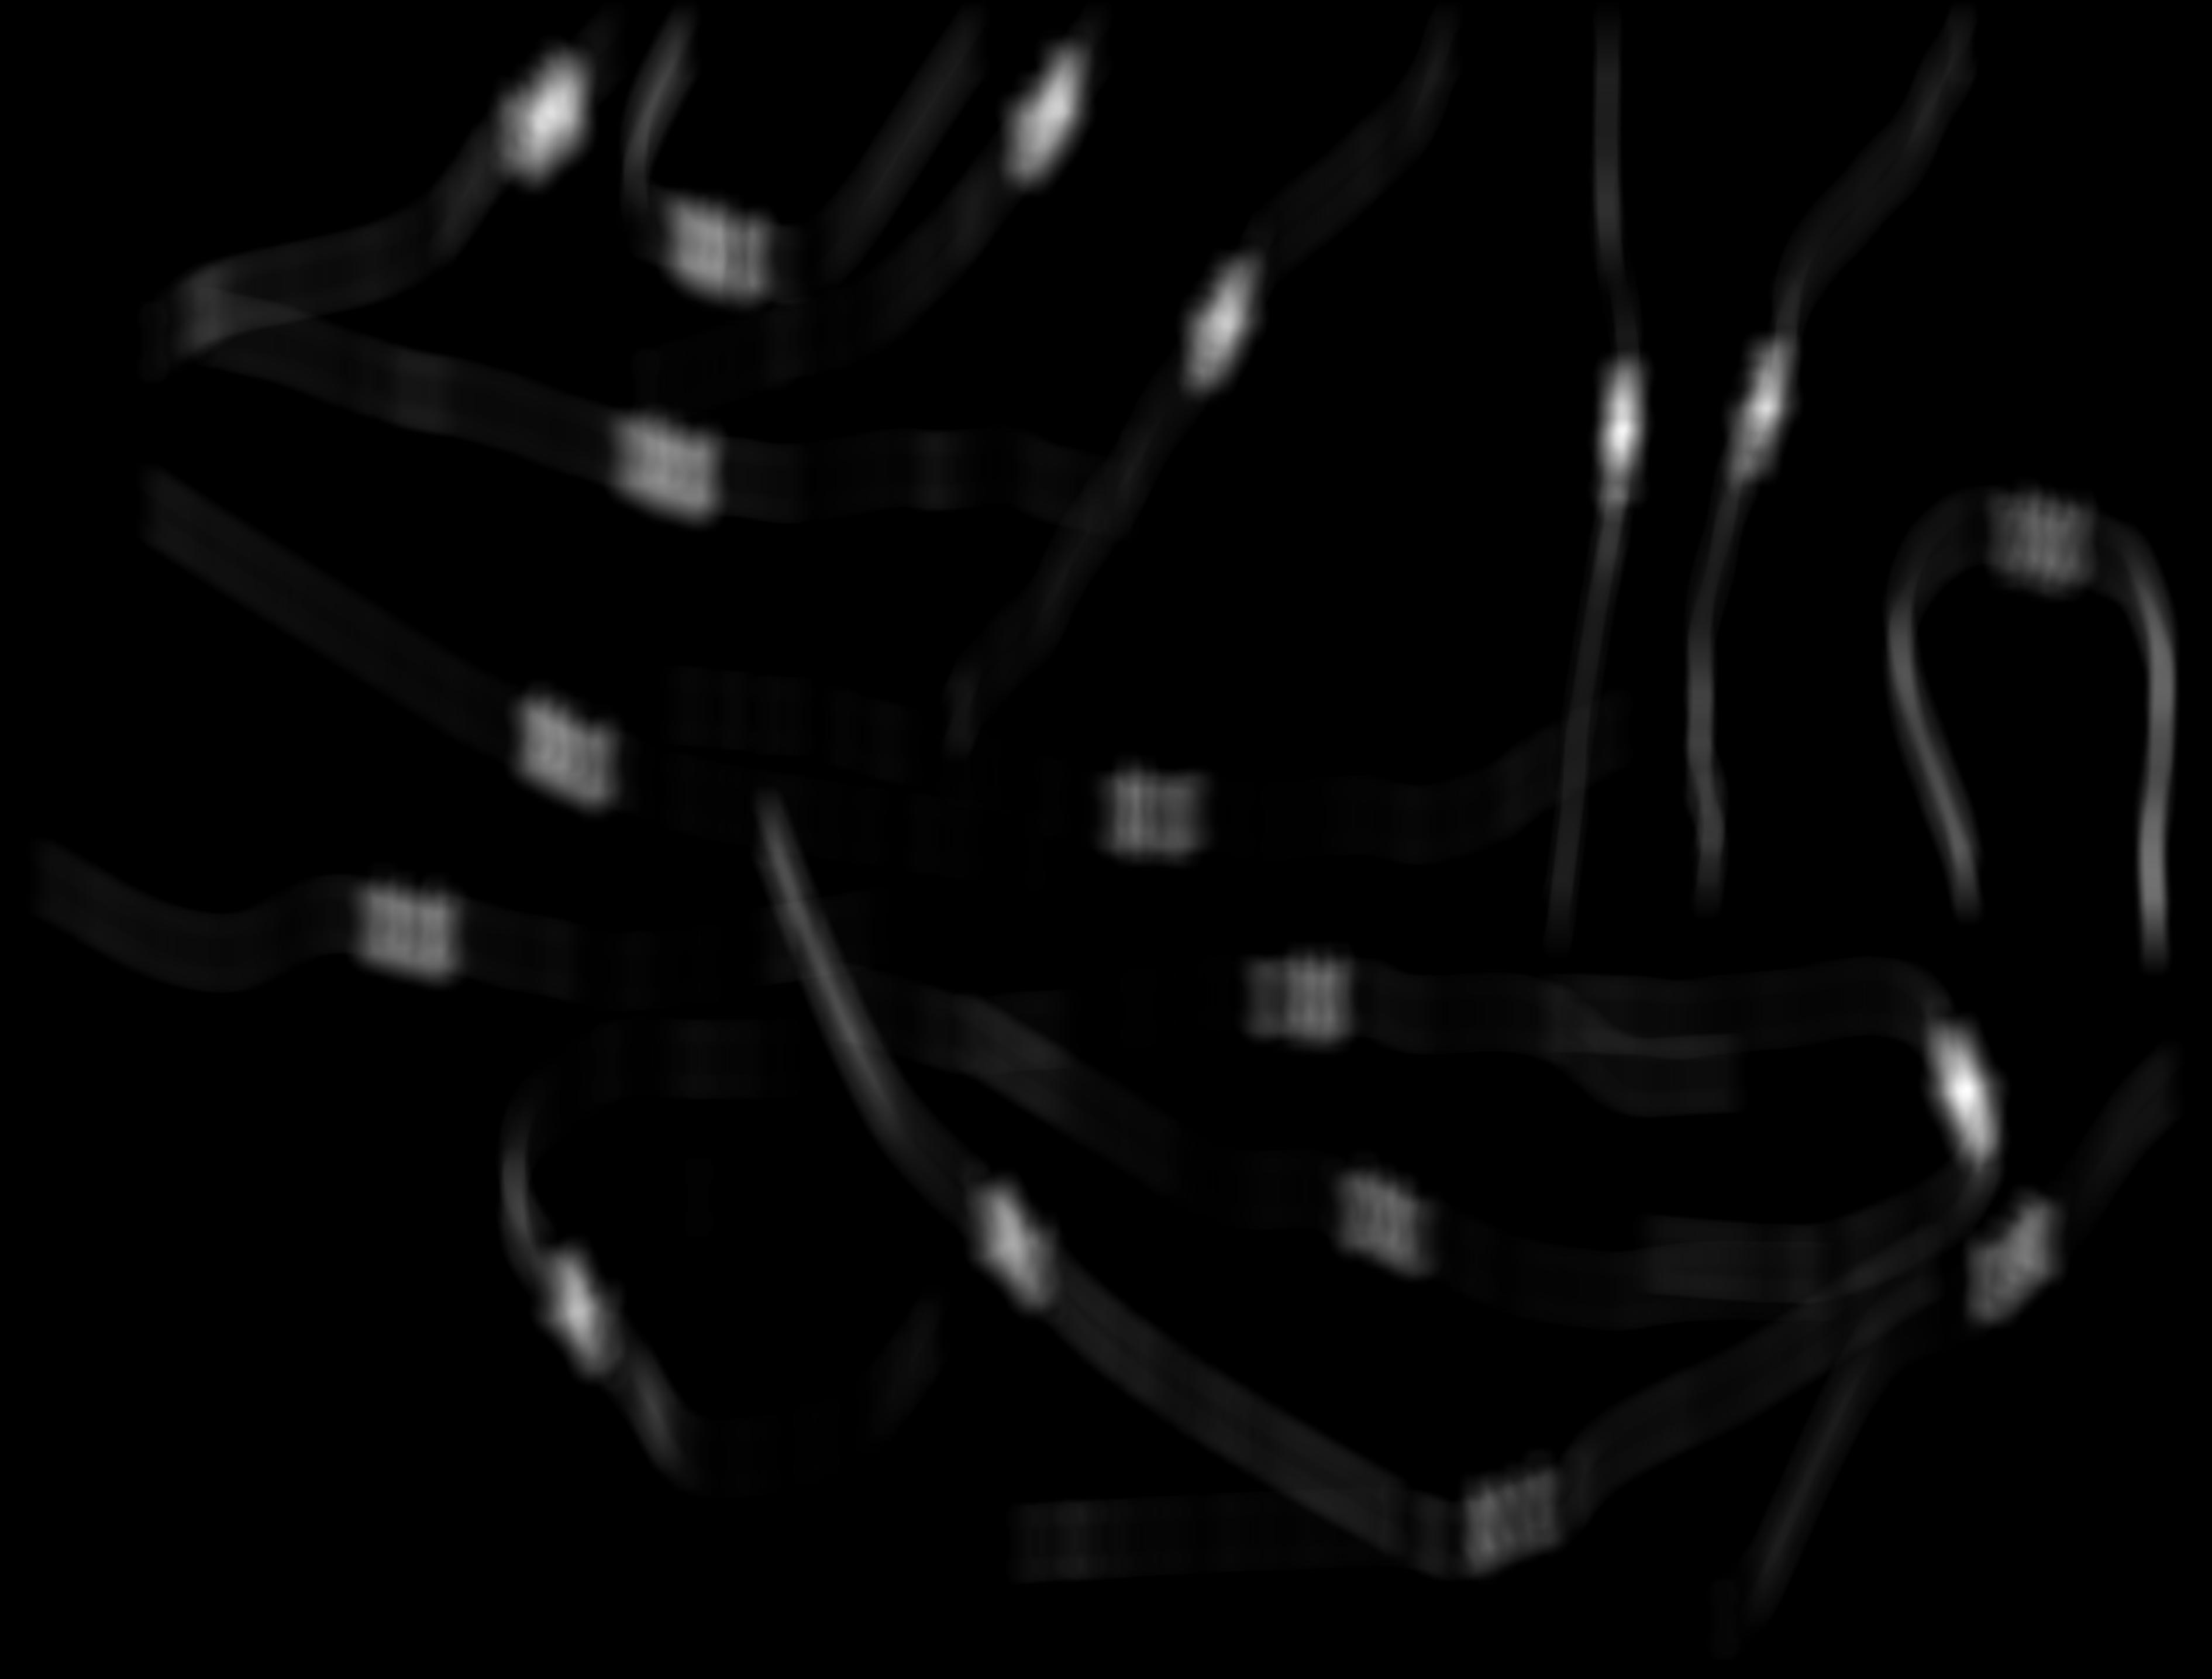
\includegraphics[width=2.2in]{images/conv90.jpg}}
\end{columns}
\end{frame}

%------------------------------------------------

\begin{frame}
\frametitle{Resistor Bounding Boxes}
\begin{center}
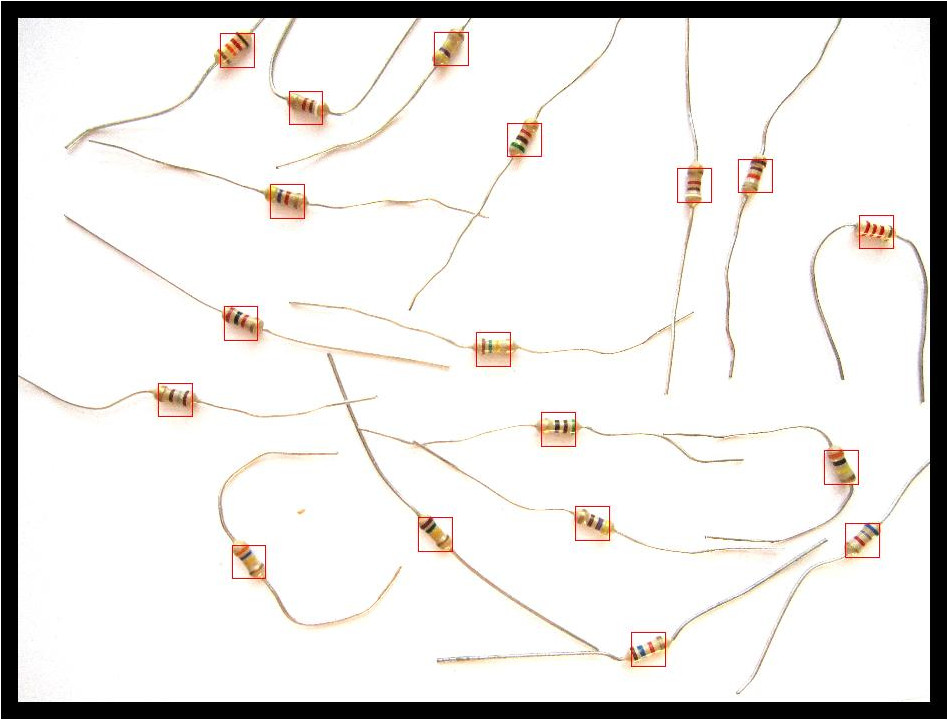
\includegraphics[width=3.5in]{images/bbs.jpg}
\end{center}
\end{frame}

%------------------------------------------------

\begin{frame}
\frametitle{Resistor Bounding Box}
\begin{center}
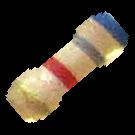
\includegraphics[width=2.5in]{images/bb.jpg}
\end{center}
\end{frame}

%------------------------------------------------
\section{Classification}
%------------------------------------------------

\begin{frame}
\frametitle{Classification}
\begin{block}{Basic Approach}
\begin{itemize}
\item Collect 3x3 mean RGB data from each color band and base resistor color 
\item Train support vector machine (SVM) classifier
\item Apply prediction to each pixel in resistor
\item Use statistical results of classification to determine resistor value
\end{itemize}
\end{block}
\end{frame}

%------------------------------------------------

\begin{frame}
\frametitle{Train Classifier}
\begin{columns}[c]
  \column{2.5in}
  	\begin{block}{}
	\begin{itemize}
	\item 11 class problem
	\item 880 training points
	\item 220 verification points
	\item Used radial basis kernel function $K(x, x') = \exp(\gamma||x-x'||^))$
	\item 5 fold cross validation
	\item Grid search for cost function (C) and $\gamma$
	\item Cross Validation Accuracy = 95.4649\%
	\item Verification Accuracy = 94.5701\%
	\end{itemize}
	\end{block}
  \column{1.5in}
  	\frame{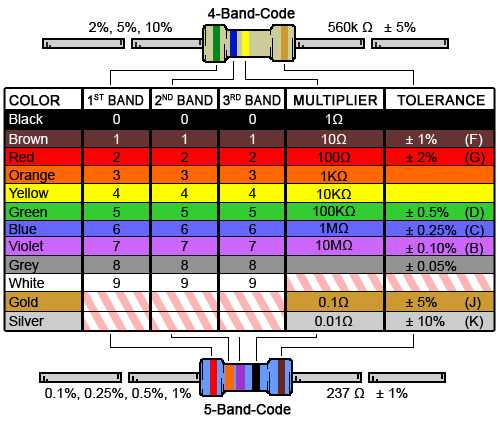
\includegraphics[width=1.7in]{images/resistor-color-chart.jpg}}
\end{columns}
\end{frame}

%------------------------------------------------

\newcommand{\ex}[2]{
\begin{frame}
\frametitle{Apply Classifier}
\begin{columns}[c]
  \column{2in}
	\frame{\includegraphics[width=2.2in]{images/example#1/masked#2.jpg}}
  \column{2in}
  	\frame{\includegraphics[width=2.2in]{images/example#1/fc#2.jpg}}
\end{columns}
\end{frame}
}

\ex{1}{1}
\ex{1}{2}
\ex{1}{3}
\ex{1}{4}
\ex{1}{5}
\ex{1}{6}
\ex{1}{7}
\ex{1}{8}
\ex{1}{9}
\ex{1}{10}
\ex{1}{11}
\ex{1}{12}
\ex{1}{13}
\ex{1}{14}
\ex{1}{15}
\ex{1}{16}
\ex{1}{17}
\ex{1}{18}

%------------------------------------------------
\section{Examples}
%------------------------------------------------
\begin{frame}
\frametitle{Resistor Bounding Boxes}
\begin{center}
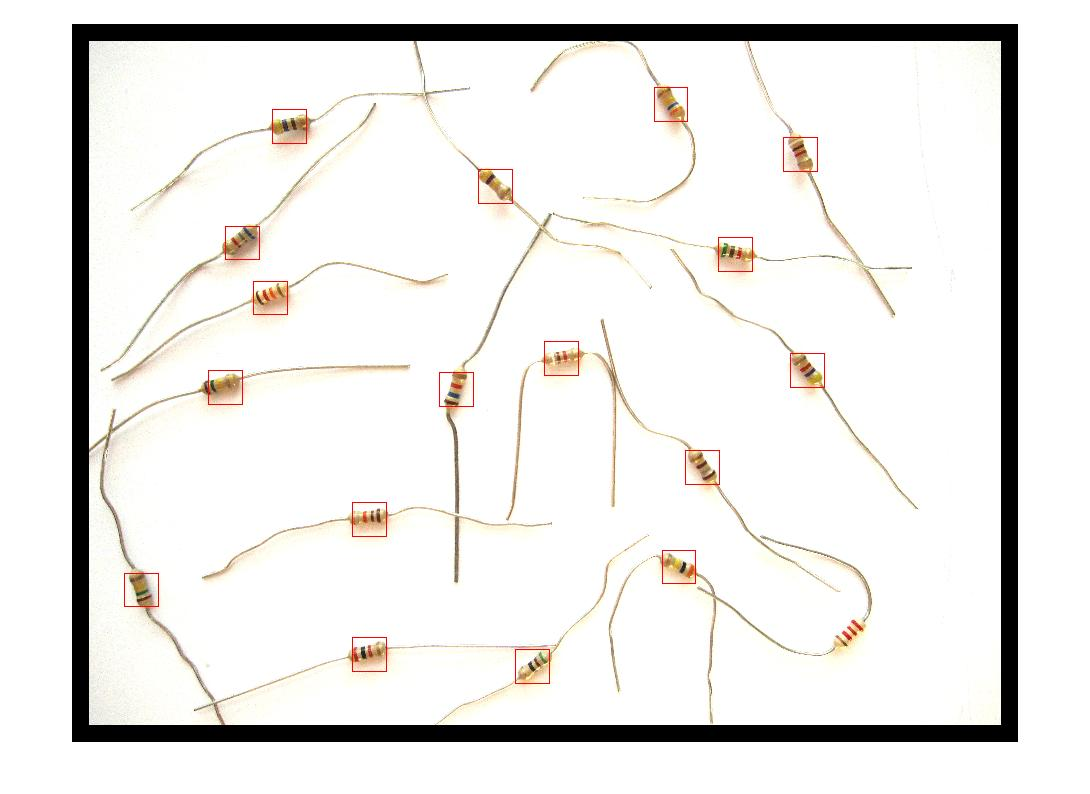
\includegraphics[width=3.5in]{images/example2/bbs.jpg}
\end{center}
\end{frame}

\begin{frame}
\frametitle{Resistor Bounding Boxes}
\begin{center}
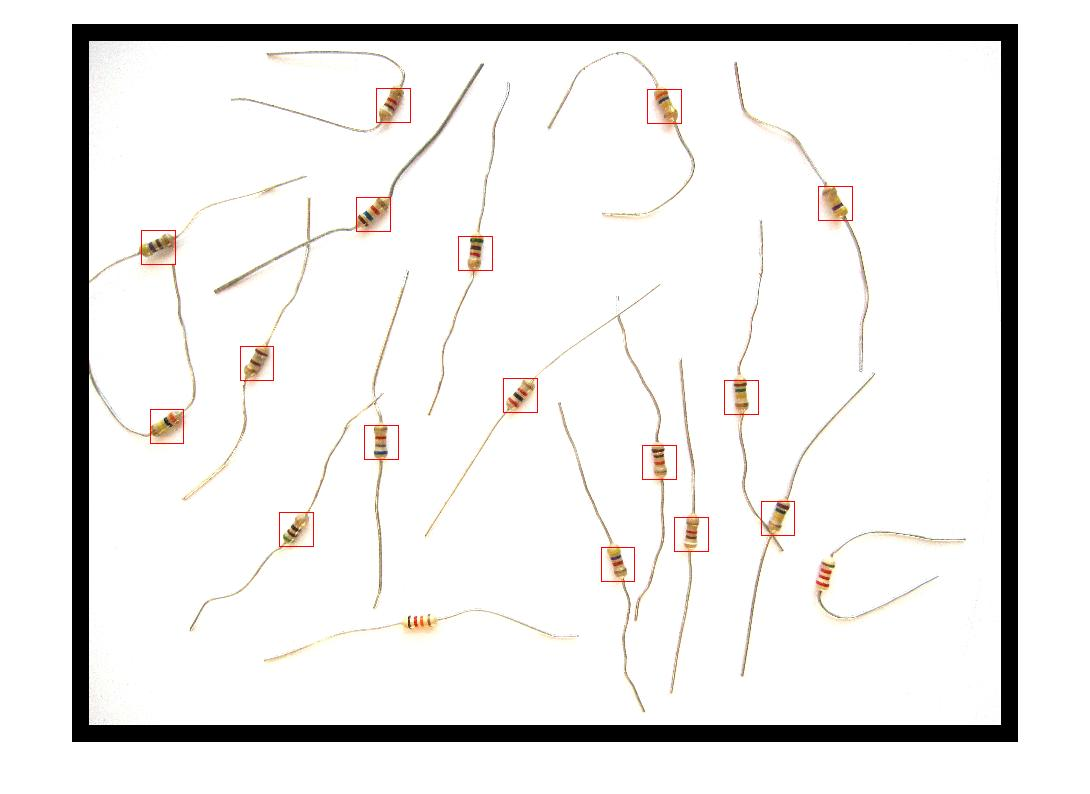
\includegraphics[width=3.5in]{images/example3/bbs.jpg}
\end{center}
\end{frame}

\begin{frame}
\frametitle{Resistor Bounding Boxes}
\begin{center}
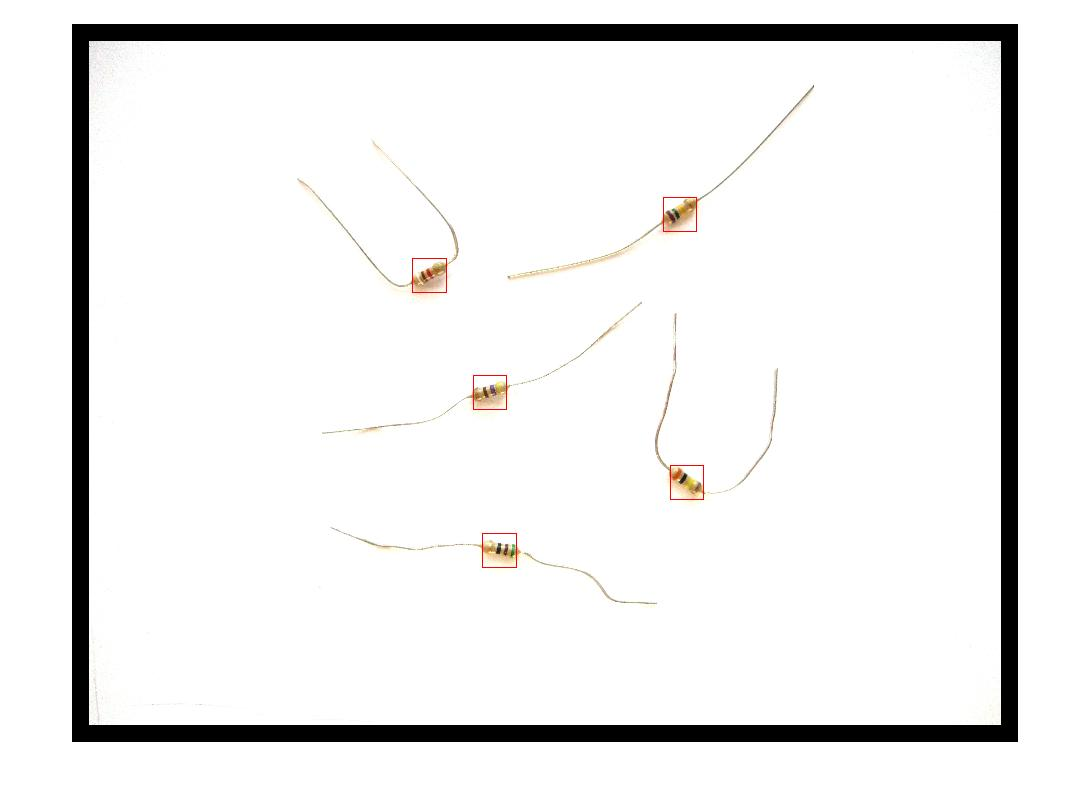
\includegraphics[width=3.5in]{images/example6/bbs.jpg}
\end{center}
\end{frame}

\begin{frame}
\frametitle{Resistor Bounding Boxes}
\begin{center}
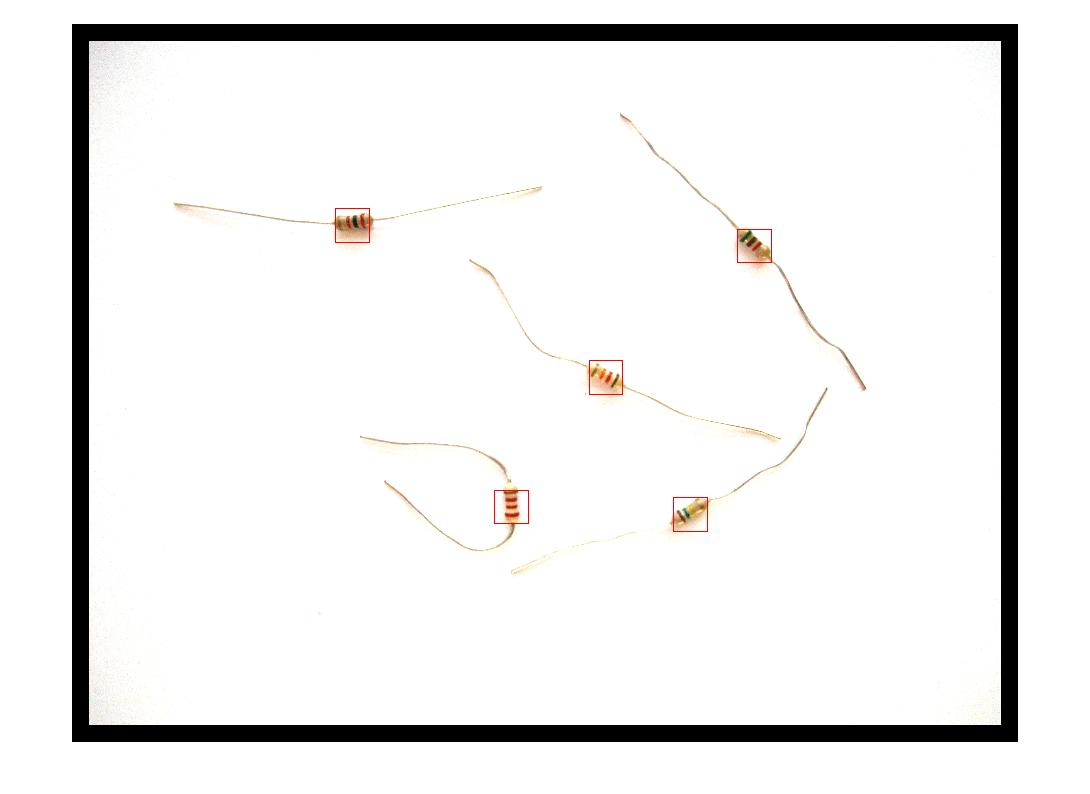
\includegraphics[width=3.5in]{images/example7/bbs.jpg}
\end{center}
\end{frame}

\begin{frame}
\frametitle{Resistor Bounding Boxes}
\begin{center}
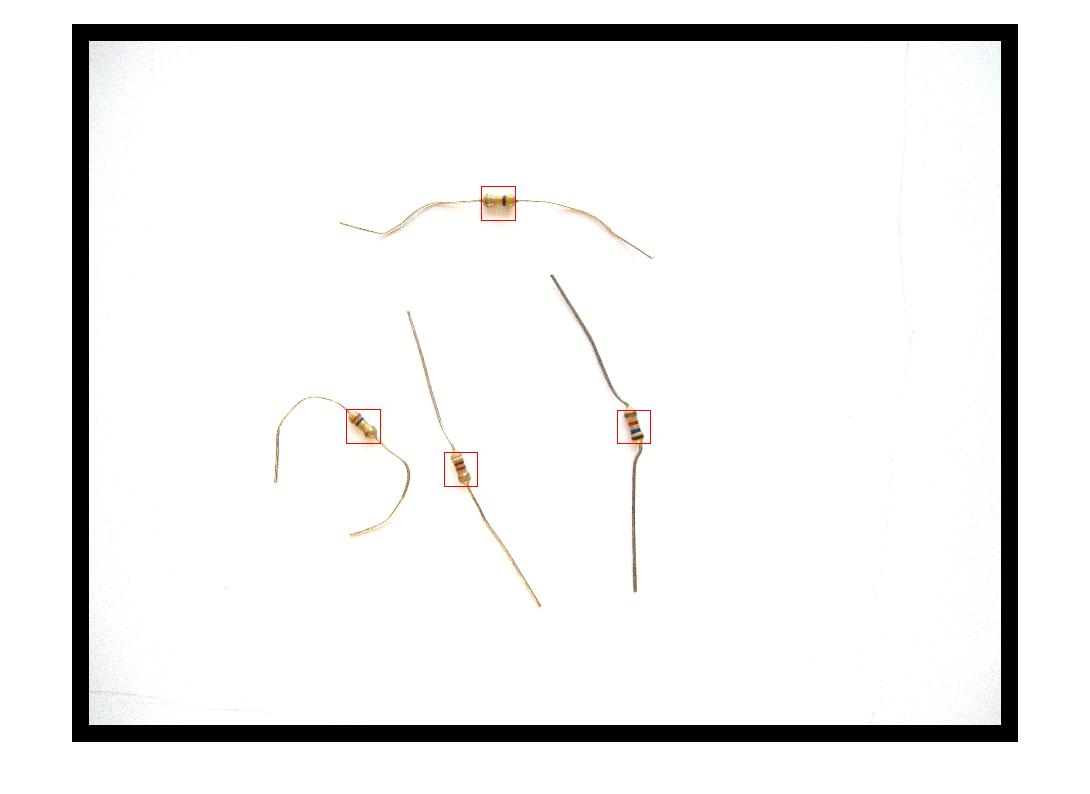
\includegraphics[width=3.5in]{images/example8/bbs.jpg}
\end{center}
\end{frame}

\begin{frame}
\frametitle{Resistor Bounding Boxes}
\begin{center}
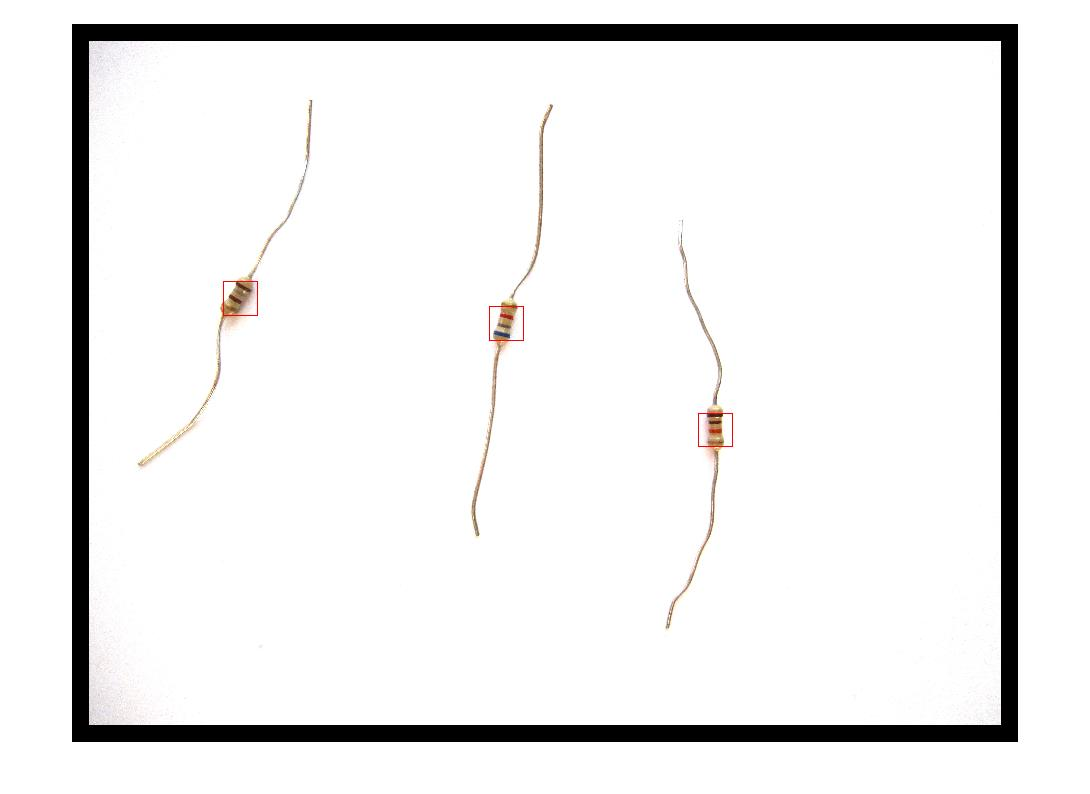
\includegraphics[width=3.5in]{images/example9/bbs.jpg}
\end{center}
\end{frame}

\begin{frame}
\frametitle{Resistor Bounding Boxes}
\begin{center}
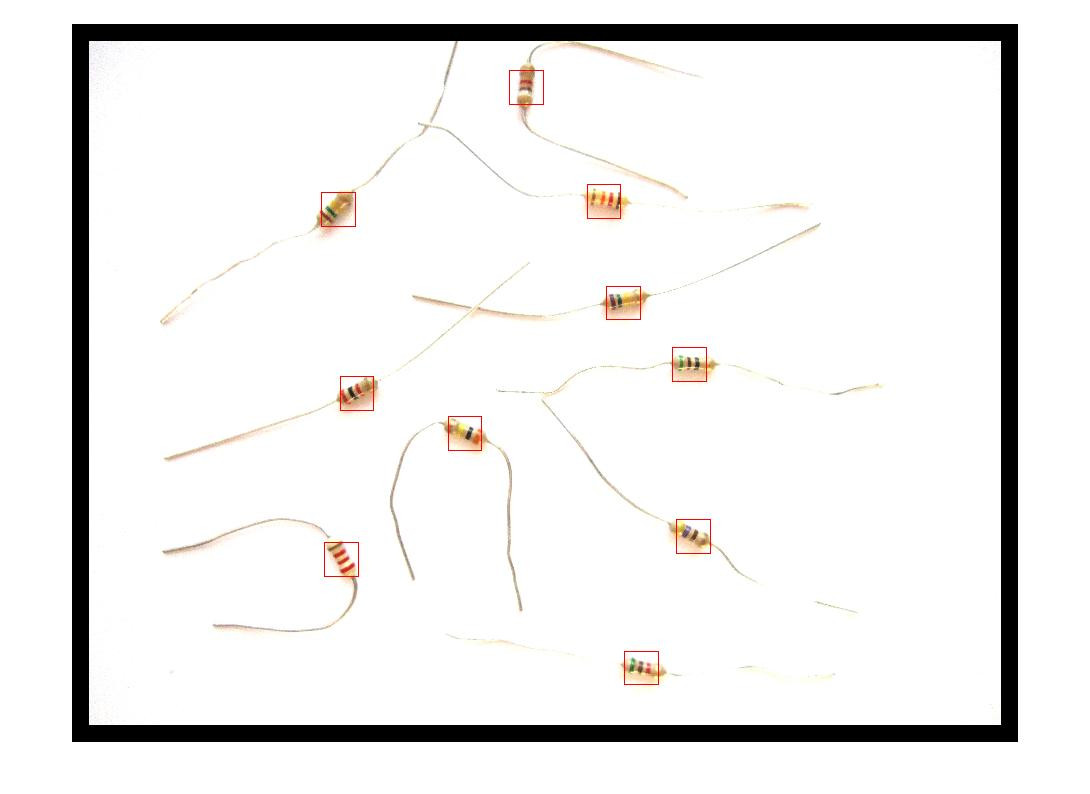
\includegraphics[width=3.5in]{images/example4/bbs.jpg}
\end{center}
\end{frame}

\ex{4}{1}
\ex{4}{2}
\ex{4}{3}
\ex{4}{4}
\ex{4}{5}
\ex{4}{6}
\ex{4}{7}
\ex{4}{8}
\ex{4}{9}
\ex{4}{10}


\begin{frame}
\frametitle{Resistor Bounding Boxes}
\begin{center}
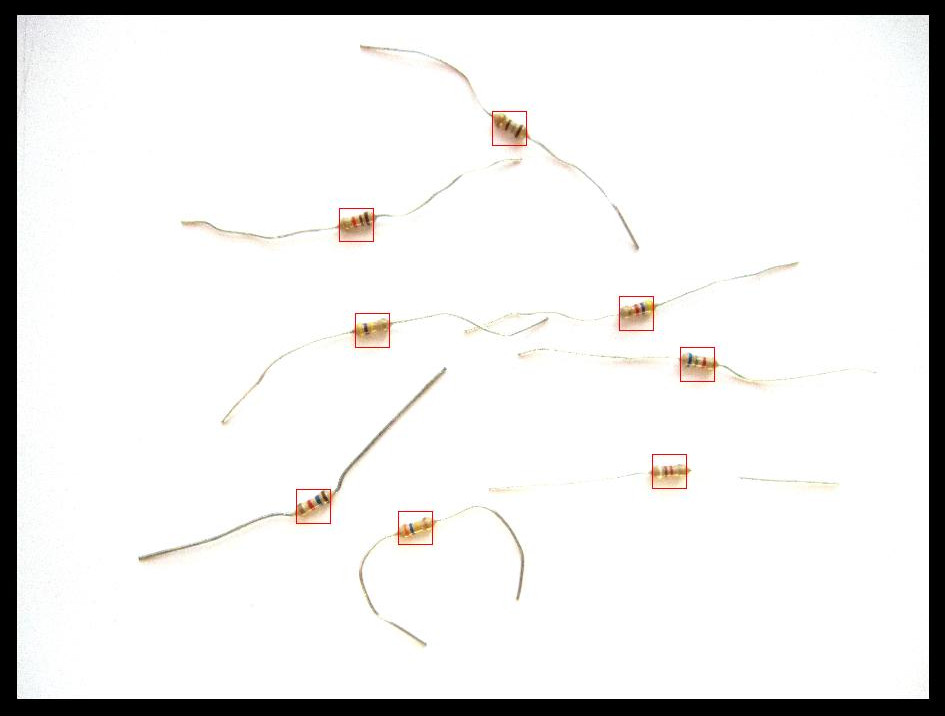
\includegraphics[width=3.5in]{images/example5/bbs.jpg}
\end{center}
\end{frame}

\ex{5}{1}
\ex{5}{2}
\ex{5}{3}
\ex{5}{4}
\ex{5}{5}
\ex{5}{6}
\ex{5}{7}
\ex{5}{8}

%------------------------------------------------
\section{Conclusion}
%------------------------------------------------

\begin{frame}
\frametitle{Future Work}
    \begin{block}{}
	\begin{itemize}
	\item Use classification data to determine color code
	\item Use line walking method and standard resistor values to improve accuracy
	\item Create augmented reality mobile app
	\end{itemize}
	\end{block}
\end{frame}

%------------------------------------------------

\begin{frame}
\Huge{\centerline{Questions?}}
\end{frame}

%----------------------------------------------------------------------------------------

\end{document} 